\section{Question 3}

\begin{question}
    Write a function in $\MATLAB$ that implements Newton's method. Your function should be of the following form:
	\begin{verbatim}
		function [p,iters] = newtonmethod(f,df,p0)
	\end{verbatim}
	where \verb+f+ is the function, \verb+df+ is the derivative, and \verb+p0+ is the initial guess, and the outputs are solution \verb+p+ and the number of iterations \verb+iters+. Use a tolerance of $10^{-10}$ to check whether the solution is close enough to 0, and have your function stop after 100 iterations if it hasn't converged. Include comments at the top of the function that explain the inputs and outputs if someone else was to use your code. Test it by finding a zero of $f(x) = \sin x$.
\end{question}

\begin{answer}
    I wrote a function as below:
    \begin{verbatim}
        %% The function newtonmethod
        % The input are the functions f and its derivative, and p0 is the intial 
        % guess of the solution. The outpout are the solution p and the number of
        % iterations iters.
        function [p,iters] = newtonmethod(f,df,p0)
            p = p0 - f(p0)./df(p0);
            iters = 0;
            while abs(p - p0) >= 10^(-10) && iters < 100
                p0 = p;
                p = p0 - f(p0)./df(p0);
                iters = iters + 1;
            end
        end
    \end{verbatim}
    Then, I tested the function using $\cos{(x)}$ with a initial guess of $\tfrac{\pi}{2}$
    \begin{verbatim}
        %% Test for a zero of f(x) = sin(x)
        f = @(x) sin(x);
        df = @(x) cos(x);
        % Test the function by evaluating it at 3.12
        [p,iters] = newtonmethod(f,df,3.12);
    \end{verbatim}
    I got a result as shown in the Figure \ref{fig:fig1}
    \begin{figure}[H]
        \centering
        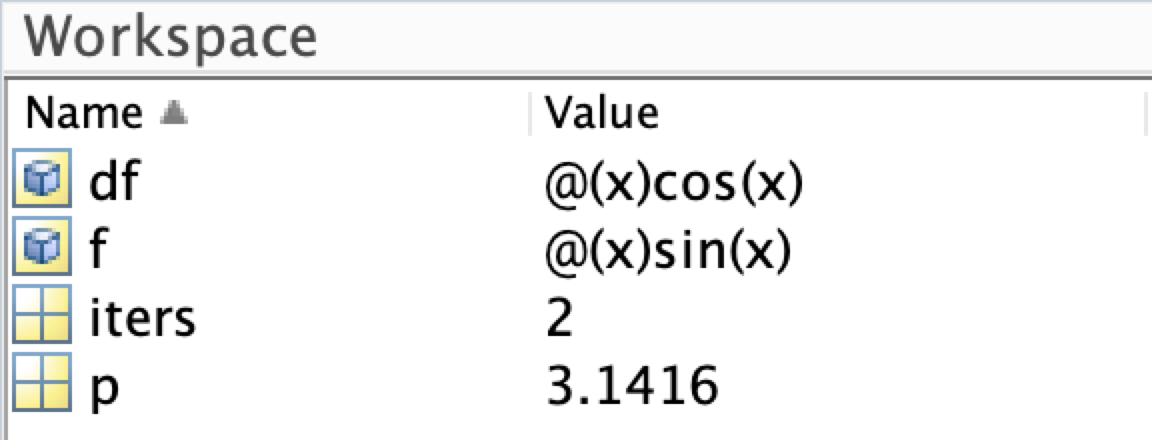
\includegraphics[width=0.8\textwidth]{Figure 1.png}
        \caption{\label{fig:fig1}Result of testing the function newtonmethod}
    \end{figure}
    The result is good since $3.1416$ is closed to the zero $\pi$ of $\sin{(x)}$, and it is also closed to our initial guess $3.12$.
\end{answer}